\documentclass[titlepage]{article}
\renewcommand{\baselinestretch}{1.5} 
\usepackage{graphicx}
\usepackage{caption}
\usepackage{textcomp}
\usepackage{subcaption}
\usepackage[margin=2cm]{geometry}
\usepackage{titling}
\usepackage{csvsimple}
\usepackage{longtable}
\usepackage{booktabs}
\usepackage{float}
\usepackage{cite}
\usepackage{lineno}
\usepackage{natbib,letltxmacro}
\LetLtxMacro\cite\citep 
\linenumbers
\newcommand{\subtitle}[1]{%
  \posttitle{%
    \par\end{center}
    \begin{center}\large#1\end{center}
    \vskip0.5em}%
}

\title{Investigating genetic correlations between female extra pair reproduction, female reproductive success and pair bond strength}
\author{Sarah Dobson sld21@ic.ac.uk\\[1cm]{\small Supervisor: Julia Schroeder }}
\date{19th December 2021}


\begin{document}
  \maketitle
  \section{Introduction}
  
  Socially monogamous species were previously thought to be genetically monogamous, but DNA analysis has shown that not all offspring are sired by the social father \cite{brouwer2019extra}. This is termed extra pair reproduction (EPR), which results from extra pair behaviour (EPB). EPP can be beneficial for males, as they can increase the number of offspring they produce. However, the benefits to female remian unclear \cite{forstmeier2014female}. Why female EPR occurs across socially monogamous species is debated amongst scientists. One explanation, called the within-sex pleiotrophy hypothesis, is that genes associated with female EPR are maintained in populations through pleiotropic effects on female reproductive traits that are under positive selection \cite{forstmeier2011female}.  Studies where the females’ social environment varied reported positive genetic correlations between female EPB and fecundity where previously no correlations were found \cite{forstmeier2011female, wang2020role}.  It is important to account for indirect genetic effects (IGEs) from the female’s social environment when looking at genetic correlations between female EPR and reproductive traits, as IGEs could bias heritability estimates \cite{radersma2021estimating}. Yet to date, no study has explicitly accounted for the females' social environment when investigating genetic correlations between female EPR and reproductive traits. One aspect of a female’s social environment that influences female EPR is the strength and stability of the social pair (dyadic) bond \cite{maldonado2021relationship}. Weak social bonds are strongly associated with increased EPB and EPR in both sexes \cite{maldonado2018linking, wang2020role}. \\

I will use association and life history data from the house sparrow population on Lundy to 1) test the hypothesis that the strength of the pair bond influences female EPR by determining if the strength of the social bond between social partners is associated with a decrease in the probability of female EPR. 2) test the within-sex pleiotropy hypothesis by testing whether female EPR is genetically correlated with measurements of female reproductive success when accounting for the strength of the social pair bond between social partners.
  
  
  \section{Proposed Methods}
  
I will determine the strength of the social pair bond by building a social network using available association data and determining the edge weight between breeding pairs. Assuming the required statistical assumptions are met, I will use a generalized linear mixed model to determine whether the strength of the social bond is associated with a decrease in the probability of female EPR. To determine if female EPR is genetically correlated with female reproductive success I will use bivariate animal models with the first response being female EPR with social bond strength as a fixed effect. Animal models allow for the incorporation of the relatedness matrix, derived from the genetic pedigree as a random effect. This random variance-covariance matrix estimates then the additive genetic effects of the response variable, and the genetic covariance, from which one can calculate the strength of the genetic correlation   \cite{wilson2010ecologist}. Typically, measures of this are confounded by environmental effects, but the Lundy sparrows have been cross-fostered systematically. This data can be used to tease apart the environmental effects from the early social environment from the genetic effects, and will allow me to accurately estimate the genetic correlations. The second response will be different measurements of female reproductive success. I will calculate female EPR as the percentage of clutches that were sired by an extra pair male.
  
  
  
 \section{Anticipated outputs and outcomes}

This project could shine light on why females in socially monogamous species cheat - a question unanswered for decades. This project should also test the hypotheses that the strength of the pair bond between social partners affects female EPR and that female EPR is maintained in the population through pleotrophic effects on traits affecting female reproductive success.



 \section{Project feasibility supported by a timeline of tasks}

Allocating tasks to specific time frames should ensure all necessary analyses can be conducted within an 8 month period (Figure 1). 

 \begin{figure}[H] 
  \centering
  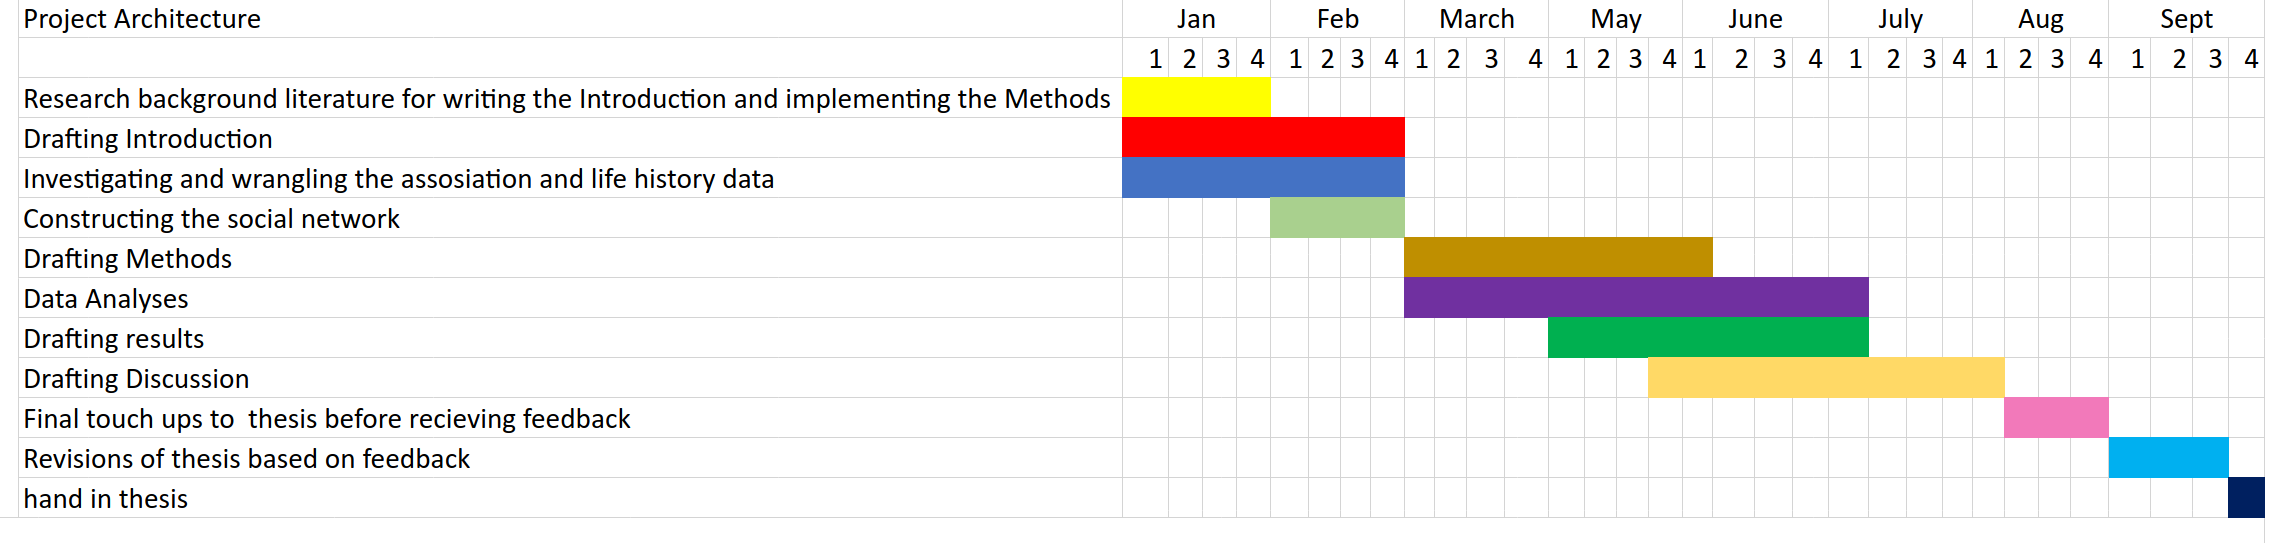
\includegraphics[scale=0.15] {Gantt.png}
   \label{Figure 1}
    \caption{\footnotesize A Gantt chart showing the proposed breakdown of tasks and the length of time needed to complete them.  Numbers 1-4 represent the weeks within each month. The coloured blocks represent each task and indicate the proposed number of weeks needed to complete each task.} 
\end{figure}







 \section{An itemized budget} 

This project does not require a budget. 



\bibliographystyle{apalike}
\bibliography{Ref}


\end{document}